\section{Vorbereitungsaufgaben}

Vorbereitungsaufgaben gibt es zu diesem Versuch nicht, jedoch empfiehlt sich, sich mit dem Oszilloskop bekannt zu machen. Dies bezieht sich eher auf Anfänger beziehungsweise auf Personen welche sich nicht \enquote{gut}
oder ausreichend bekannt mit dem Gerät fühlen. 
\paragraph \to Erzeugung einer Sinuswelle und heran- sowie herauszoomen und Ablesen der Amplitude 
und/oder eine Erzeugung einer Rechteck-Schwingung wie in Abbildung \ref{Abbildung3}.

\begin{figure}[H]
    \centering
    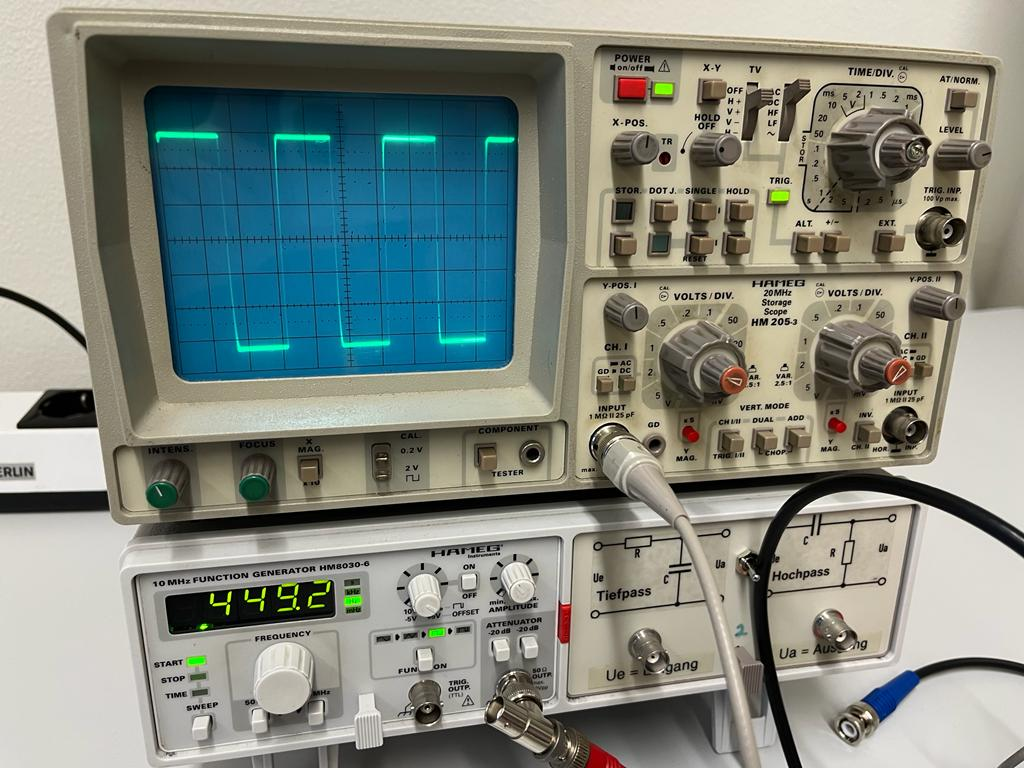
\includegraphics[width=80mm]{bilder/Ab3.jpeg}
    \caption{Bild einer Erzeugten Rechteckschwingung.\label{Abbildung3}}
\end{figure}
